\section{SN比}
式\ref{eq_Jitter}の分母を求めるために、測定したノイズと波高差を使って、信号対雑音比であるSN比の電圧依存性を調べた。
SN比は値が大きいほど、ノイズの影響が小さいと評価することができる。
\begin{equation}
    \sigma_j = \frac{\sigma_n}{\left|\frac{dV}{dt}\right|} = \frac{\sigma_n}{\left|\frac{S}{t_r}\right|} = \frac{t_r}{\left|\frac{S}{\sigma_n}\right|}
    \label{eq_Jitter}
\end{equation}

%\subsection{SN比の測定結果}
以下の図\ref{fg:PIN_SNvsBias}にPINのSN比の電圧依存性を、図\ref{fg:APD_SNvsBias}にAPDの電圧依存性を示す。
PINとAPDともに、図\ref{fg:PIN_MPVvsBias}と図\ref{fg:APD_MPVvsBias}のように、信号の大きさの電圧依存性と似た形になっていることがわかった。
これは、増幅層を入れることで、ノイズは大きくなってしまうが、それ以上に信号の増幅率の寄与が大きいため、LGAD検出器は増幅層がない半導体検出器と比べて時間分解能が向上すると考える。

\begin{figure}[h]
    \begin{minipage}[b]{0.5\linewidth}
        \centering
        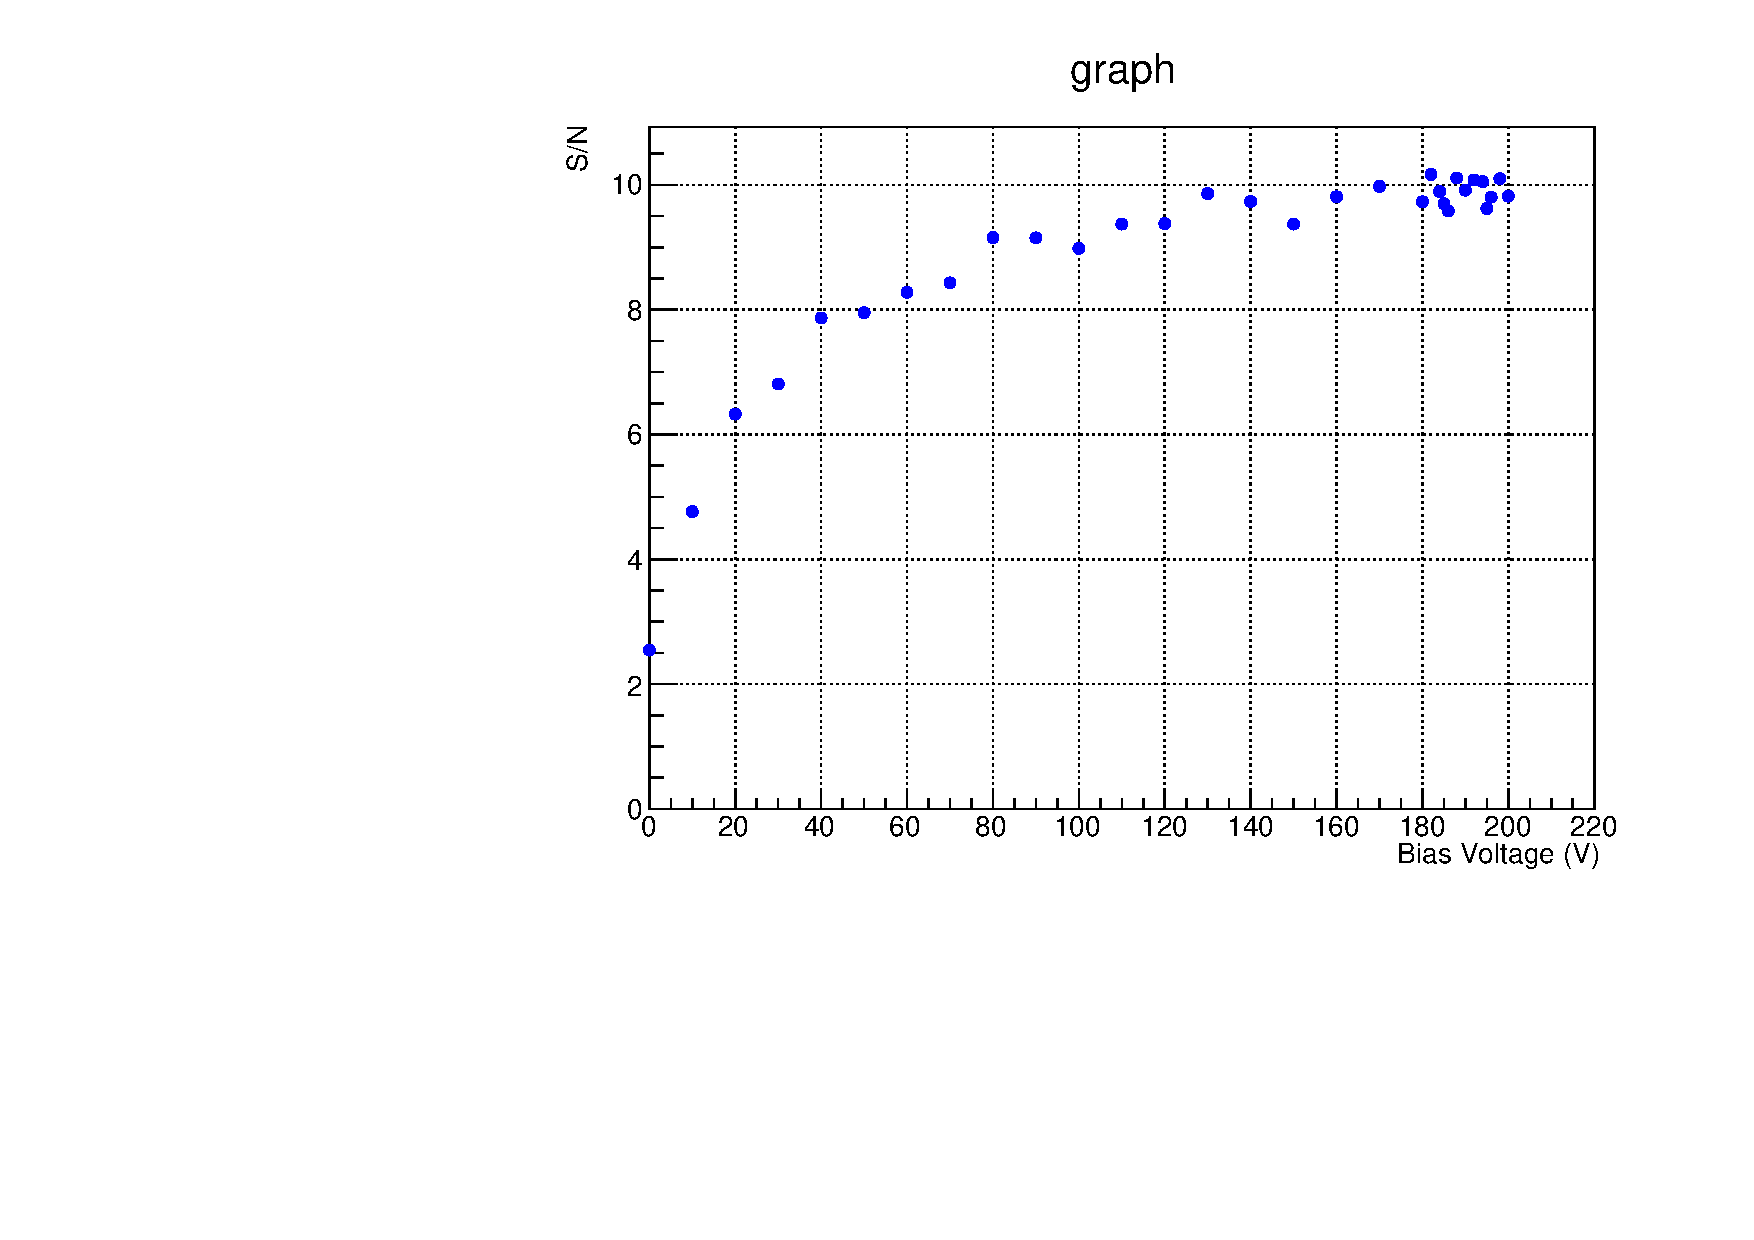
\includegraphics[width=8cm]{fig/graph/SN_pad1ch_PIN_ver2_temp_126_20231220.pdf}
        \subcaption{PINのSN比の電圧依存性}
        \label{fg:PIN_SNvsBias}
    \end{minipage}
    \begin{minipage}[b]{0.5\linewidth}
        \centering
        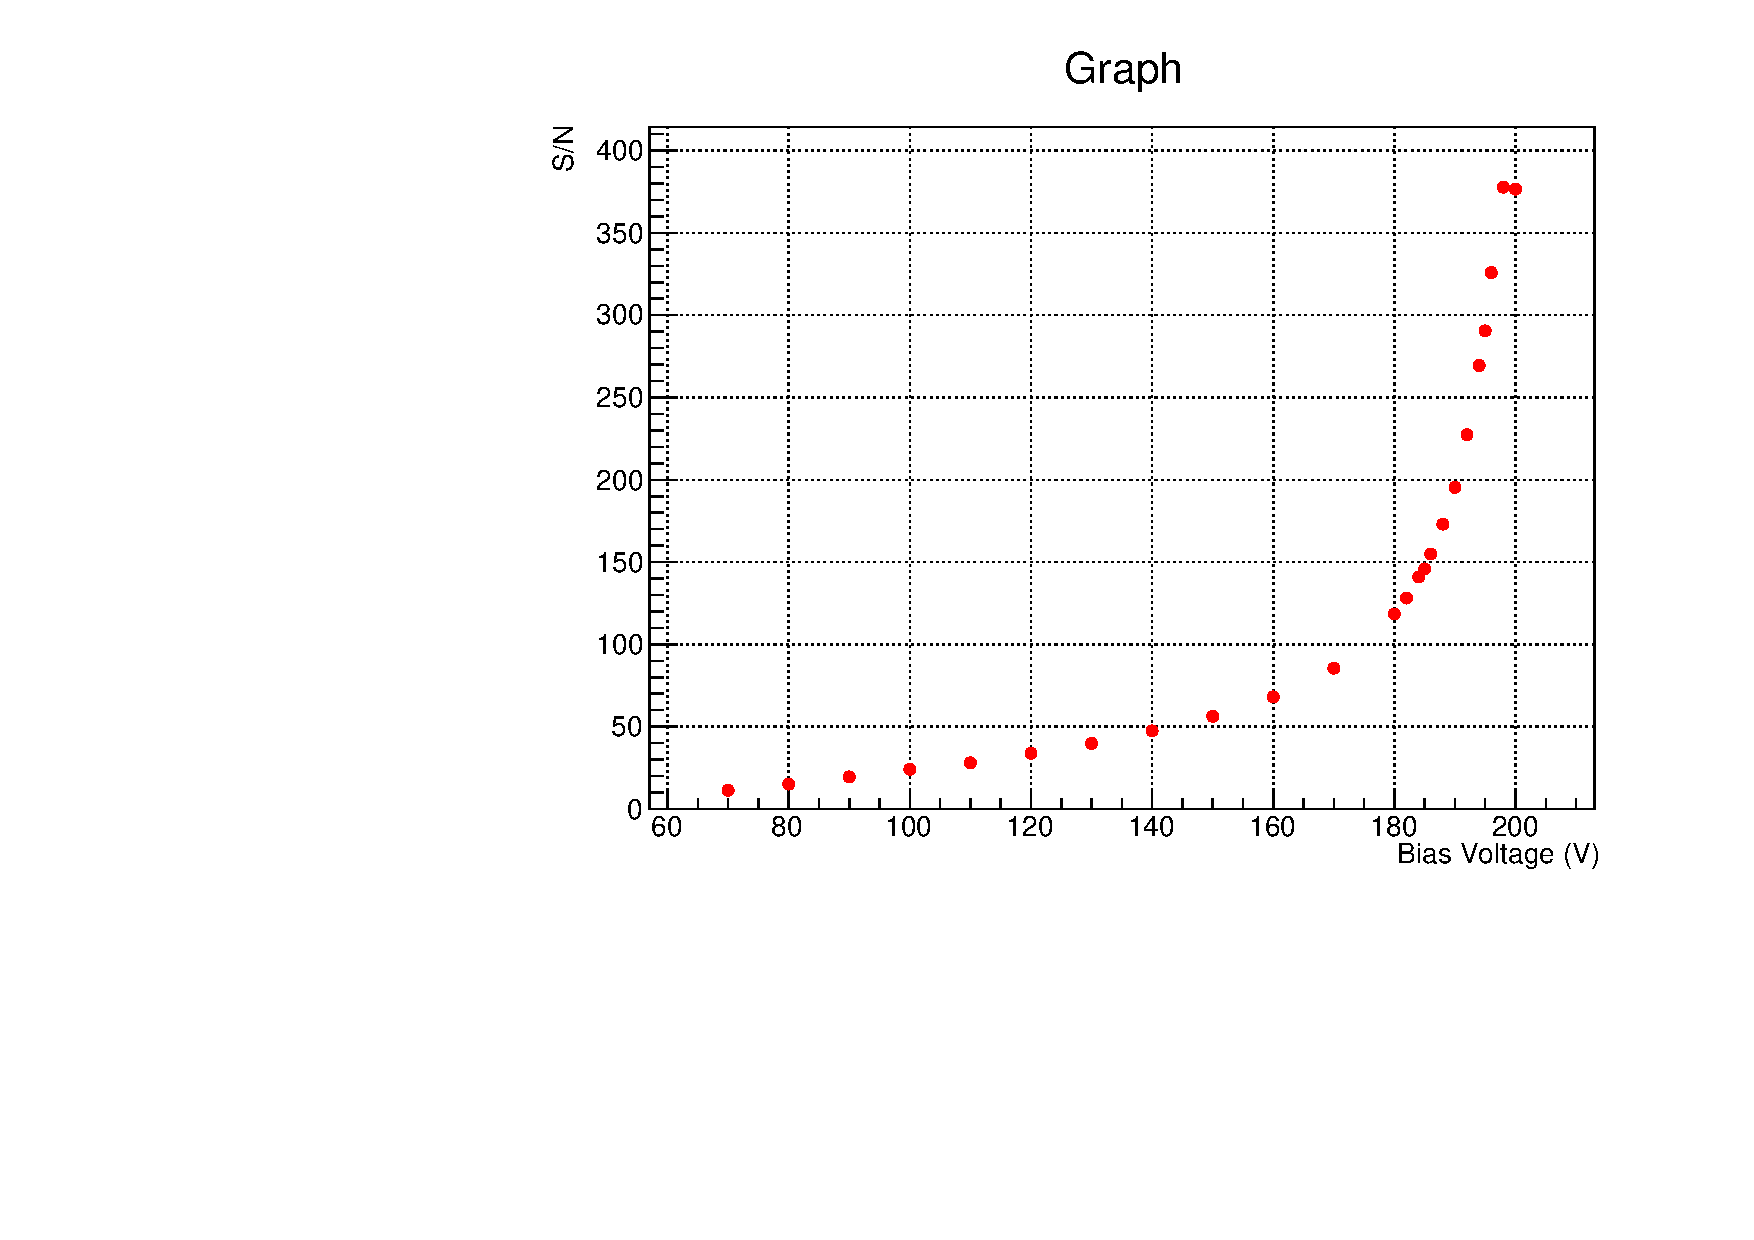
\includegraphics[width=8cm]{fig/graph/SN_pad1ch_APD_ver2_temp_126_20231220.pdf}
        \subcaption{APDのSN比の電圧依存性}
        \label{fg:APD_SNvsBias}
    \end{minipage}
    \caption{信号雑音比(SN比)の電圧依存性\\横軸が電圧で縦軸がSN比  (a)がPINで(b)がAPDのグラフ}
\end{figure}


%APDのSN比がPINと比べてどのくらい向上するかを調べるために、図\ref{fg:Noise_TresovsBias}に、SN比のAPDとPINの割合の電圧依存性を示す。
%また、時間分解能が良い時のSN比を調べるために、時間分解能の電圧依存性も同時にプロットした。
%時間分解能が良い電圧領域でのSN比の割合が、12倍から33倍になっていることがわかった。
%増幅層を入れることで、ノイズは大きくなってしまうが、それ以上に信号の増幅率の寄与が大きいため、LGAD検出器は増幅層がない半導体検出器と比べて時間分解能が向上すると考える。
%
%\begin{figure}[h]
%    \centering
%    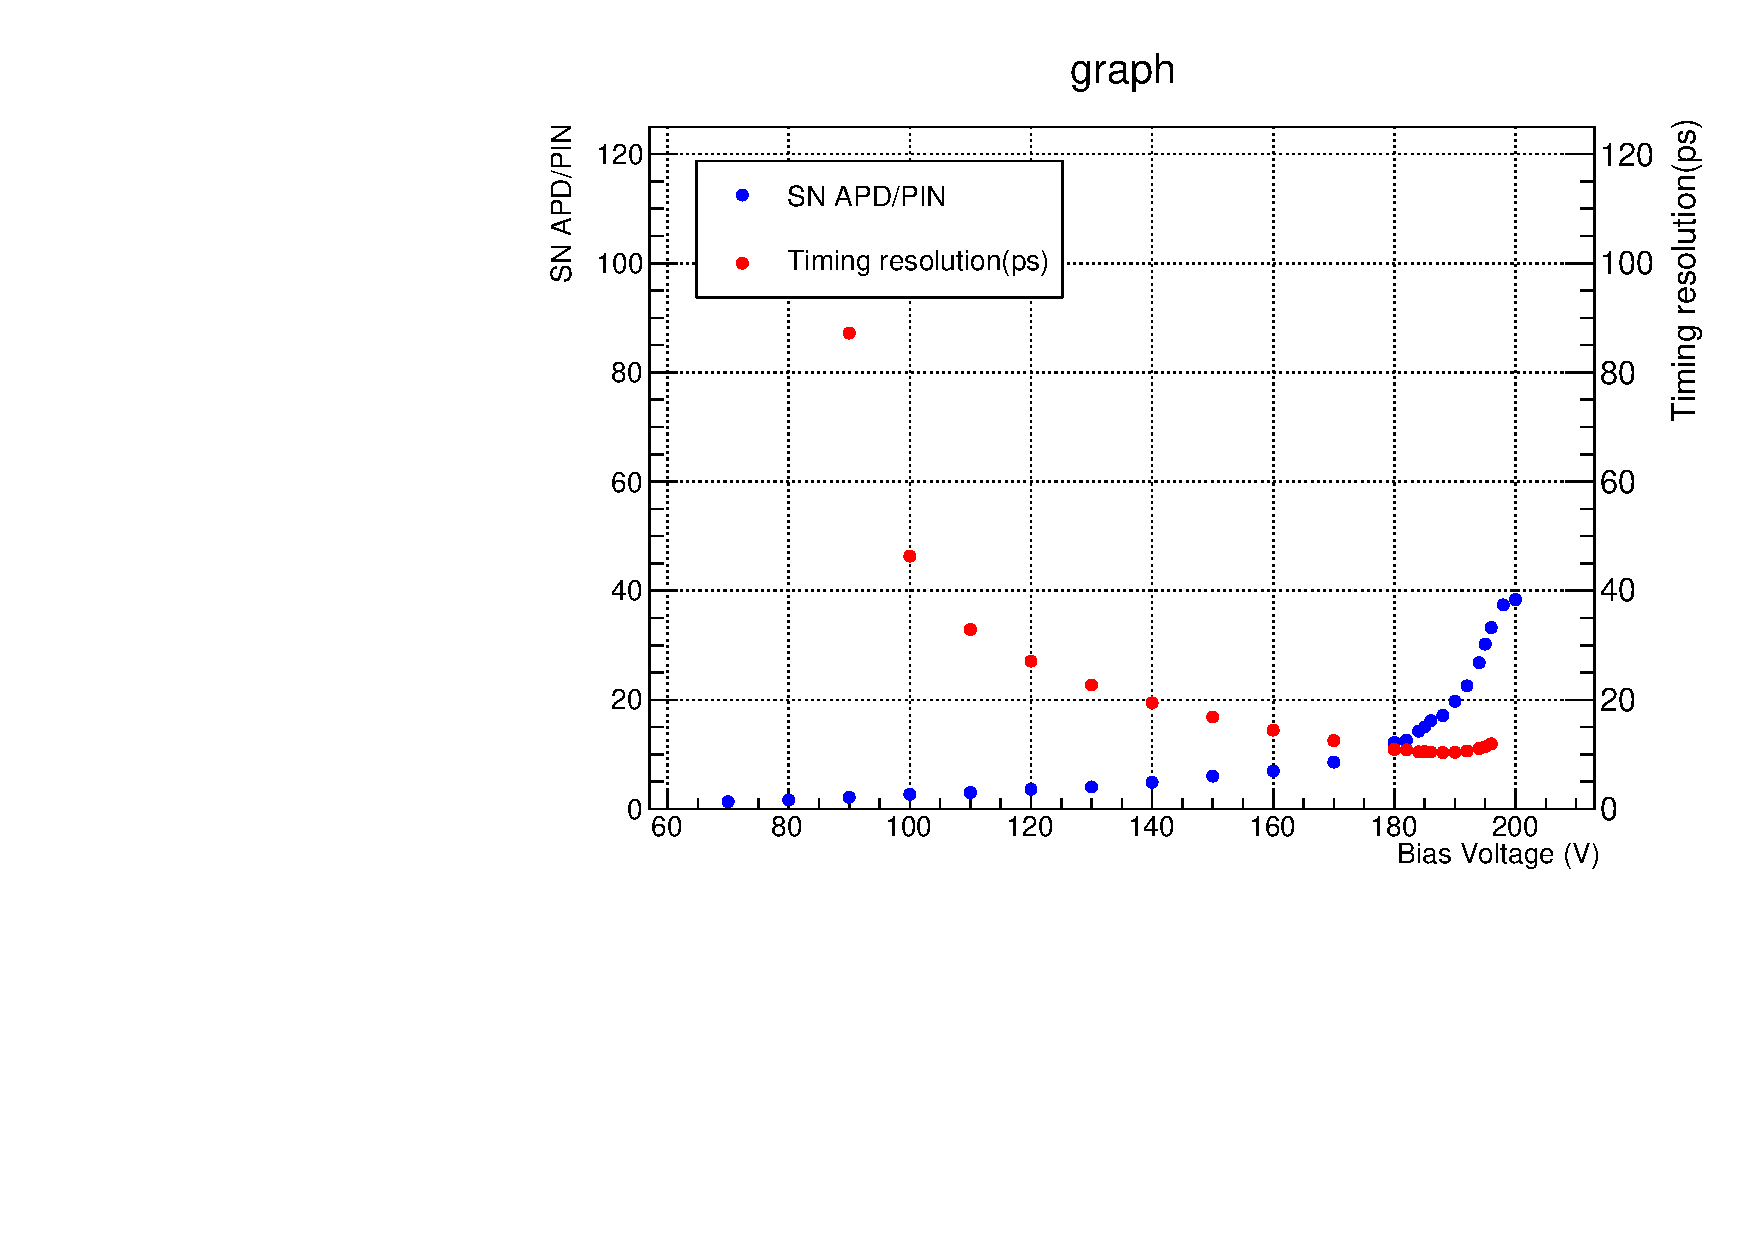
\includegraphics[width=8cm]{fig/graph/SNraito_Treso_pad1ch_ver2_temp_126_20231220_APD_PIN.pdf}
%    \caption{SN比のAPDとPINの割合の電圧依存性}
%    \label{fg:Noise_TresovsBias}
%\end{figure}





